\documentclass[draft,12pt,titlepage]{article}
\usepackage{sd}

\title{Stadium Traffic}
\begin{document}
\maketitle
\frontmatter
\abstract

\newpage

\tableofcontents
\newpage

\mainmatter
\section{Introduction}
\subsection{Overview}
Stadium Traffic aims to reduce the carbon emissions from people going to and from sports
games. In particular, our project will focus on the Philadelphia Eagles and Phillies stadiums.
We aim to build a model that can be used to quantify the carbon emissions generated due to
people coming to and going from games. We will then develop solutions to reduce the
number of people coming by cars or leave over longer time period and develop a traffic
routing algorithm, aiming to reduce the carbon emissions from idling cars waiting to leave
the stadium. We will test these on our model to find a successful combination. If we can get
the cooperation of Phillies/Eagles and Philadelphia Police Department, we hope to work with
them to implement the results of our project.

\subsection{Motivation}
All of us have been to large gatherings like sports games, concerts or conferences and can
therefore relate to the traffic problems when everyone is trying to leave at the same time at
the end of the event. However, what most people don’t realize is the environmental effect of
this traffic. Our project aims to find solutions to reduce this traffic and hence reduce the
emissions while cars idle in parking lots trying to leave.
The project is focusing on the Philadelphia Eagles and Philadelphia Phillies stadiums. Sports
events draw huge crowds at peak traffic hours and are therefore a great instance on which to
model our project. The Eagles are also undertaking a Go Green! initiative, which is a push
towards becoming more environmentally conscious. Some initiatives that they have taken are
the use of renewable energy sources for their power consumption and using cups and plates
made from recycled materials. We believe that we can get the support of the Eagles for our
project, as it can be part of the Go Green! initiative and further reduce the carbon footprint of
the stadium.
When the football or baseball game ends, everyone tries to the leave the stadium at the same
time. Although traffic police conduct the traffic, they do it in a haphazard way. Furthermore,
the decision of which gates to be open and which ones to remain closed is also done using
intuition rather than any efficiency-maximizing algorithm. We saw this inefficient process as
an opportunity to develop an algorithm to reduce car idling time and carbon emissions.

\subsection{Project Goal and Objectives}
Although the overarching aim of our project is to reduce carbon emissions due to people
going to/from the sports games, we broke this down into certain specific and measurable
objectives:

\begin{enumerate}
  \item Develop a comprehensive model of transportation to and from the stadium.
  \item Quantify the total emissions due to transportation to/from games.
  \item Develop a tool to simulate the emissions impact of various initiatives to reduce
private transportation usage (e.g. offering a discounted drink to someone who rides
the SEPTA).
  \item Create an algorithm to optimally route exiting vehicle traffic according to total
emissions generated.
  \item Develop a method for the Philadelphia traffic police to implement the traffic routing
recommendations of our project.
\end{enumerate}

The success of each of the objectives can be measured and how we would measure the
success is stated below:

We would consider a success model one that takes inputs such as trip distribution, number of
attendees, start and end time and produces outputs such as average idling time and number of
cars.

The aim of the project is to reduce carbon emissions, so we need to be able to measure and
quantify carbon emissions from idling cars.

Our model should be able to quantify the effect of different incentives on carbon emissions so
that we can test different strategies and find the optimal combination.

Optimal routing of traffic can impact carbon emissions from idling cars, so we need to create
an algorithm that can be constraint optimized. A working algorithm can help the traffic police
conduct traffic in a more organized manner.

Having a front-end system that can be used by the Philadelphia Police will allow our
algorithm to be implemented and hence allow our project to have an impact. Therefore we
need a computer or phone application that can be used by the police while conducting traffic.

\subsection{Constraints}
With any ambitious project, there are always certain constraints and we have recognized the
constraints of our project so that we can be prepared to work around them.

The main constraint is the cooperation of the Philadelphia Phillies/Eagles and
Philadelphia Police Department because without their cooperation we cannot implement our
project. However, our advisor Dr. Huemmler has good relationships with both organizations
and has been trying to get their support for the project.

Another constraint is the team’s lack of experience with transportation engineering.
Since the project involves the understanding, modeling and optimizing of transport systems,
this would be a constraint. However, we have taken an initiative to get the help of Professor
Vukan Vuchic, a senior professor in transport engineering, and began familiarizing ourselves
with relevant transport systems concepts under his guidance.

Finally, our last constraint is the data collection required to build a representative
model. However, we have been trying to get the required information from the Phillies,
Eagles, and other government departments.

\section{Discussion of Previous Work}
\subsection{Group Members' Prior Work}
One of our group members, Felipe Ochoa, has had extensive experience working with Penn
Transit to improve the dispatching efficiency of their bus operations around campus. This
work has allowed for in-depth understanding of queuing theory and demand generation,
which will be extremely useful in our module about fans taking cars to the game. Using
elements of the prior project, combined with additional concepts from traffic engineering, we
will be able to develop an accurate model.
\subsection{Scholarly Work}
\subsubsection{Phoenix, Arizona Planning Authority}
The planning authority in Phoenix, Arizona, MAG, undertook an extensive project in 2011 to
develop a model to understand transit movement to planned special events in the region. \cite{kuppam11} Our
chosen topic, sports games, falls under the category of a planned special event. Their paper
identifies the proportion of special events patrons who utilized light rail v. alternative modes
of transportation and how they thought about modeling demand and modal choice for this
event. We hope to utilize their thinking to support our own idea generation on how to model
sports patrons. Our project will be going above and beyond their project by specifically
looking at sports games, narrowing in on a specific type of “planned special event” and
developing a comprehensive understanding of modeling travel related to these events.

\subsubsection{Transportation Engineering Basics}
This is a textbook that clearly describes how a travel demand model is created through the
components of Trip Generation, Trip Distribution, Mode Choice and Trip Assignment. \cite{murthy01} We
will be trying to understand the motivation for Trip Generation, which is based on Trip
Purposes as specified in the book. The two purposes relevant for our project are HBO (Home
Based-Other) and NHB (Non-Home Based). We hope to extend the information in the book
on these purposes and develop a trip generation model that accurately reflects the proportion
of these HBO and NHB trips are to sports game in order to quantify the demand generated.
We also hope to use the Trip Assignment information contained in the book and push the
envelope to understand Trip Assignment for sporting events.

\subsection{Trip Generation}
This database details various data patterns related to Trip Generation.\cite{ite08} We will be able to use
the information contained herein, specifically the information related to the special events
travel, e.g. sports games and movies. We hope to extend the work by conducting first-hand
research to grow our dataset and make our predictions and algorithms that much more
accurate.

\section{Strategic Plan/Structure}
The driving principle behind our strategic plan can be summarized as ``Benchmark, then
improve.'' Our project will therefore first focus on computing `sensible' emissions values for
an average game, and will then develop a full model to quantify the impact of different
policies that could be put in place. In engineering terms, we are first calculating the
equilibrium or ``trim'' condition and then we will focus on disturbances away from it.
\subsection{System Proposed Approach}
The approach to both problems will of necessity be similar, and our aim is to design our
solution to the first problem with a great deal of flexibility so that it may be readily adapted
for use in the second phase of the project. Our phase 1 model will have five main components
that correspond to the four steps of the UTMS plus a GHG calculator. The blocks described
below correspond to the block diagram shown in figure \ref{mainsystem1}.

\begin{figure}[htp]
  \centering
  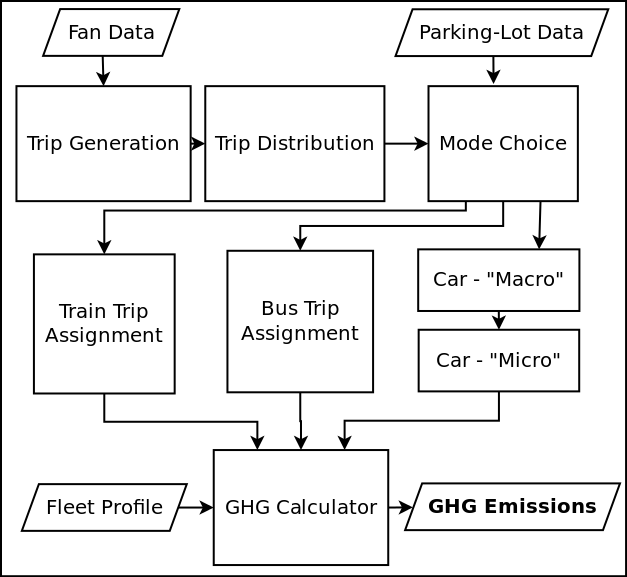
\includegraphics[width=.3\textwidth]{fullsystem1.png}
  \caption{System block diagram of our phase 1 model}
  \label{mainsystem1}
\end{figure}

\begin{description}
  \item[Trip Generation] \hfill We will need to gather data on the geographic distribution of the fans that attend the games. We hope to obtain a good amount of data from the Eagles to aid in this section. Absent that data, we will have to resort to theoretical models commonly
used in the industry, such as the Gravity Model. We will also be gathering data on
timing of the trips, either through direct observation, or ideally from already existing
records.
  \item[Trip Distribution] \hfill This step in the modeling is straightforward, since we know that fans are traveling to and from the stadium (or a nearby parking lot).
  \item[Mode Choice] \hfill This phase involves matching each trip in the database to a mode of travel (i.e. Car vs. SEPTA vs. Bus). We plan on using parking-lot data to estimate car use, and, if possible, get station-level information directly from SEPTA. A variety of theoretical models exist to help validate the gathered data. 
  \item[Trip Assignment] \hfill Is the selection of the specific lines, streets, highways, and stations that each trip will follow. At this stage, we will break the model into subsystems for each of the possible means of transportation.
    \begin{description}
      \item[Trains] \hfill A great deal of information is available on the website regarding
lines and schedules that we have used to build a software representation of the
network. With some well-established linear optimization algorithms, we will be able
to model the exact path taken for every trip assigned to SEPTA trains.
      \item[Buses] \hfill Schedules and stops are also available at www.septa.org, and we will merge
this database with the information available on Google Maps to obtain location data.
There are also well-established algorithms we can use to model the paths of every
trip.
      \item[Cars] Our car model will be split in two:
        \begin{itemize}
          \item At a "micro" level, we will model the road network in and around the stadium
parking lot based on existing databases complemented with hand-input data that
we extract from maps and planning documents. This portion will be used to
model the exiting cars, since we believe the congestion at the end of a game
results in substantial GHG emissions.
          \item At a "macro" level, we will use the same TAZs as in the trip generation phase,
and calculate a sample path to the stadium based on highways and main roads.
We will have to encode the network of such roads and use our own algorithms.
Alternatively, depending on the resulting number of TAZs, and subject to special
authorization, we could use the Google Maps API to programmatically retrieve
routing information.
        \end{itemize}
    \end{description}
  \item[GHG Calculator] \hfill This subsystem will be a memoryless function mapping a trip to
an estimated emissions value. Our preliminary assumption is that trips taken on
public transit contribute no additional GHG, since we are taking the bus and train
schedules as given. For cars, there are a multitude of published methods for
estimating emissions. We will have to estimate a fleet profile (average age and size)
to use one of these models. We expect that it will be a function of total highway
distance/time, local street distance/time, and idling time. When properly built, the
output from this subsystem will be our first main deliverable.
\end{description}

For the second phase of the project, as mentioned above, we will seek to leverage as much of
the modeling work from phase one as possible. The goal for this phase will be to focus on
converting the existing model into a usable simulator. A key objective will be incorporating a
variety of inter-system feedback mechanisms that will allow for a more accurate model.
There will of course be a trade-off between complexity and accuracy at this stage that we will
have to explore. Since there may be limited opportunities to validate our model (until the next
season begins), a key performance metric will be the consistency of results, which in
technical terms, means that the system should reject small disturbances in the inputs.
Conceptually, changing the base fare for SEPTA or increasing the cost of parking by small
amounts should not result in wildly different behavior. This sensitivity will be a key measure
we will use in determining the right level of complexity to build into the model.

Some examples of feedback mechanisms we are considering at this stage are:

\begin{description}
  \item[Congestion] \hfill If a fan spends 45 minutes stuck in the parking lot unable to
move, we expect that fan to be more likely to take the train for the next game. A more
detailed discussion of the fan model lies below.
  \item[Scheduling] \hfill If SEPTA notices trains traveling fuller on game days, they may
choose to alter schedules in the future.
  \item[Uncertainty Effects] \hfill As fans try different modes of transportation, they may refine
their predictions of travel times and convenience.
  \item[Fleet Composition] \hfill We suspect the fans that are most likely to start using
public transit may have cars with above-average fuel efficiency, whereas the fans that
take their trucks to tail-gate parties will likely continue to use their less-efficient cars.
These effects would alter the fleet profile and hence average emissions calculations.
\end{description}

Regardless of what feedback loops we ultimately incorporate, we will have to build a model
of the fans' utilities, to capture the effects of the various incentive schemes on trip generation
profiles. At this stage we expect we will be using an agent-based technique for this
subsystem, which will have as inputs the TAZs and some demographic data. Cooperation
from the Eagles will be important in fine-tuning this part of the model.

The expanded model can be seen in the block diagram in figure 2. We have included the
incentive structure as an input in the diagram. We expect to make a GUI for this input to the
model.

\subsection{System Specification}
Our end system must have a GUI that can be used by Eagles management to input proposed
incentives and that will output the projected change in GHG. The input must be intuitive and
friendly enough that it does not require a manual for a user of average computer literacy to
learn to use it in 10 minutes or less. Additionally, once a user is familiar with the interface,
varying parameters on a proposed incentive program should not require more than 2 minutes
of the user's time.

The back-end must be flexible and have a documented API so that a software developer may
write extensions to the model (e.g. different incentive types) or refine sub modules (e.g. a
more efficient traffic assignment subsystem) without having to modify the other components
of the software. Additionally, the model must be fast enough so that initial estimates of GHG
emissions under certain incentive schemes may be computed within 5 minutes. In addition,
detailed logs and reports (e.g. emissions over time graphs) should be accessible to a more
knowledgeable user through the same GUI.

The program must handle improper input robustly and must be able to deal with exceptions
and errors gracefully. Specifically, a user of average computer literacy should be able to
understand error messages, and, in a worst-case scenario, should be able to simply reset the
application to restore functionality.

The subsystem specifications are laid out in table \ref{specs}
\begin{table}[htp]
  \centering
  \caption{Specifications table}
  \label{specs}
  \begin{tabular}{%
    >{\raggedright}p{.11\textwidth}%
    p{.74\textwidth-6\tabcolsep\relax}%
    >{\raggedright\arraybackslash}p{.15\textwidth}}
    \firsthline
    \bfseries Module & \bfseries Qualitative Requirements & \bfseries Quantitative Performance Requirements \\ \hline
    Trip Generation & Interface with a database of TAZs and (if
possible) a database of sanitized user data in strict XML format. 

Output a list of trips specifying the origin and time of each one. &
    $5\,s$ per $50,000$ trips \\
    Trip Distribution & Pass through the list from the trip generation
module. & N/A \\
    Mode Choice & Read in sanitized parking-lot data in SQL, station-level usage information, and TAZ demographic profiles. Assign a mode choice to each entry in the the list from the trip distribution module. 
 
Output a vector of the different trips in each category and 
summary statistics for each mode (e.g. utilization percentage). &
    $10\, s$ per $50,000$ trips \\ 
    Trains & Read in a line and schedule XML database
and accept an input of trip origin and time pairs. Calculate the most direct path to the stadium for each trip , subject to capacity
constraints. Output summary statistics and trip list. & $1\,$min per 50,000 trips \\
    Buses & As above, with its own (larger) database. The trip profiles must not specify stop-by-stop, but rather total distance, to within 5\% error. & $1\,$min per 50,000 trips \\
    Cars & (See below) & $1\,$min per 50,000 trips total \\
    Cars - Micro & Accept the list of trips and read in a
database of the road network in and around the stadium. Compute total distance and idling time per car to reach the highways/main roads. & \\
    Cars - Macro & Accept the same list of trips as above and compute total highway and secondary road times across all trips. Optionally interface with the Google Maps API. & \\
    GHG Calculator & Process the outputs from the trip assignment modules and compute an overall level of GHG emissions. & $10\,s$ per 50,000 trips \\
    \lasthline
  \end{tabular}
\end{table}
\subsection{Hardware and Software Requirements}
\subsubsection{Hardware Requirements and Design Approach}
The hardware requirements for this project will feature towards the tail end of the project.
The end-user (be it the Eagles/Phillies or the policemen directly traffic), will be receiving a
finished piece of software from us, which would require specialized hardware to deal with it.

In order to make the software/algorithm we create generalizable, we will be utilizing a
popular hardware choice of either a personal computer or a portable device (iOS/Android). The choice will be made upon further discussion with the Eagles and at this time we are
unable to provide reasons for a technical hardware choice.

\subsubsection{ Software Requirements and Design Approach}
The software we create will be created primarily in Matlab and Python. The requirements we
have from our software will be as follows:

\begin{description}
  \item[Modularizable] \hfill We should we able to switch out one implementation of the train model, for instance, and replace it seamlessly with another, more efficient implementation.
  \item[Scalable] \hfill It should be able to handle a large number of inputs and not break under scale. It will have to deal with tens of thousands of fans inhabiting the model.
  \item[User-Friendly] \hfill We want the final output, or GUI, to be extremely user-friendly and it should be operational without a manual.
\end{description}

The software here isn’t a complement to the hardware; in fact the actual crux of our project is
based on the software. As a result, defining the specific functions of our software would be
equivalent to defining the scope for this project, which is done through this 1st Project Report.
In summary, we will be looking to create a model that takes in data about demand generation
and incentives and uses that to determine the modal usage of transportation to Eagles games.
Finally, we will be using the model to determine the amount of time cars idle and based on
expected CO2 emission rates, we will be determining the impact of the incentives inputted
into the model. We will also be developing a module to incorporate feedback, allowing for
``state'' in our model (i.e. prior experiences impact future choices).


\addtocounter{subsection}{1} %\subsection{Test and Demonstration}
%\subsubsection{Test}
%\subsubsection{Demonstration}

\subsection{Schedule}
The schedule consists of the different tasks that we estimate we will need to accomplish in
order to have a successful project. The tasks can be broken up as those falling into

\begin{itemize}
  \item Planning and design
  \item Creating the required subsystems
  \item Integrating the subsystems into one system
  \item Implementation.
\end{itemize}

Each task is assigned to only one individual although others may also be working on the
tasks, but the assigned individual is accountable to get it done correctly and on time. Based
on the Gantt chart and schedule it is clear that we aim to work consistently over the course of
the year to meet the milestones (course requirements) and also aim to get some work done
over winter break so that we don’t fall behind schedule.

Our current status is that we are ahead of schedule in some tasks, whereas we are behind
schedule in other tasks. However, this is not as much of a concern to us as being completely
behind schedule because we can alter resource allocation to reconcile the variance and bring
the project back on schedule.

The two areas where we are behind schedule are:

\begin{enumerate}[(a)]
  \item Working with the Philles/Eagles and
  \item Working with the Philadelphia Police Department.
\end{enumerate}

This can be attributed to the major constraint mentioned in the introduction. Dr. Huemmler
has been trying to get us in touch with them, but so far they have not been very cooperative.
However, we cannot allocate more time to this to bring us back on schedule until we have
established contact. But after that we can devote more resources to the subtasks to bring it
back on schedule.

The tasks where we are ahead of schedule are the calculation of carbon emissions. We over-
estimated the time it would take to research and find the necessary data.

\section{Preliminary Results}
{\huge MISSING}

\addtocounter{section}{1} % \section{Lessons Learned}

\section{Equipment/Fabrication/Software Needs}
We do not have any need for specialized equipment or software. The software we will be using is either publicly available, or available at Penn. We expect that our production version of the model will not depend on commercial tools.

\addtocounter{section}{1} % \section{Conclusions and Recommendations}

\section{Nomenclature}
\begin{table}[htp]
\centering
\begin{tabular}{%
    >{\raggedright\bfseries}p{.1\textwidth}%
    p{.9\textwidth-4\tabcolsep}}
  API & Application programming interface. A means to programatically access a database, such as that of Google Maps.
  GHG & Greenhouse gases. We mostly mean Carbon Dioxide, but we use the term GHG since emissions are highly correlated across types in this application. \\
  MAG & Maricopa Association of Governments. It is in charge of transportation planning for Phoenix and it surroundings. \\
  SEPTA & Southeast Pennsylvania Transit Authority. Manages the commuter rail, the
subway, trolley, and bus systems in and around Philadelphia \\
  SQL & A type of database that is commonly used. \\
  TAZ & Traffic analysis zone. Used in modeling the UTMS. It involves dividing a geographical area into units that have sufficiently similar transit and demographics to treat as one for the purposes of the model. \\
  UTMS & Urban Transportation Modeling System. A commonly used framework to model traffic demand and flows. \\
  XML & A structured file format that is human-readable and easily parseable \\
\end{tabular}
\end{table}

\makereferences

\makebibliography

\section{Financial Information}
We expect our project to incur minimal cost. At this time, the only foreseeable expenses are the cost of transportation to the stadium. Depending on how we refine the user needs after our meeting with the Eagles, we may have to purchase a mobile device on which to prototype our model interface.

%\section{Ethical Issues}

\appendix

\ssection{A Documented Module of Code}

\begin{verbatim}
#! /usr/bin/env/python3

"""
stations.py reads in an xml file containing a list
of station elements with name and url subelements.
It fetches those urls and tries to extract the lines
serving those stations from the websites. It updates
the xml and saves the updated list into a (potentially)
new file.

usage: $ python stations.py xml-file-name [output-name]

"""

import xml.etree.cElementTree as ET
import urllib.request
import re
from urllib.error import HTTPError


class Station:

    LINES_RE = re.compile("<p>This station is served by:<br ?/?>"
                          "(.+?)</p>", re.DOTALL)
    BREAK_RE = re.compile("<br ?/?>")
    PARKING_RE = re.compile('<table[^>]*>\s*<tr>\s*<td[^>]*>'
                            '<h2 class="normal">Parking</h2>'
                            '.*</table>', re.DOTALL)

    def __init__(self, element):
        self.element = element
        assert (self.element.find('url') is not None)
        self._html = ''
        self._lines = []
        self._parking = []

    @property
    def url(self):
        return self.element.find('url').text

    @property
    def html(self):
        if not self._html:
            self.update_html(self.url)
        return self._html

    def update_html(self, url):
        # UTF-8 encoded checked by hand on a couple of urls
        try:
            self._html = urllib.request.urlopen(url).read().decode('utf8')
        except HTTPError as e:
            self._html = "HTTP Error #" + str(e.code)

    @property
    def lines(self):
        if not self._lines:
            self.update_lines()
        return self._lines

    def update_lines(self):
        section = self.LINES_RE.search(self.html)
        try:
            section = section.group(1)
        except AttributeError:  # No match found
            self._lines = ["REGEX ERROR"]
            return
        section = section.strip()
        section = self.BREAK_RE.sub("\n", section)
        # subbing <br>s may result in double newlines,
        # and hence blank "entries"
        # That's why composition below is filtered
        self._lines = [s.strip() for s in section.splitlines() 
                                                  if s.strip()]

    def set_lines(self):
        lines = self.element.find('lines')
        if lines is None:
            lines = ET.SubElement(self.element, 'lines')
        for line in self.lines:
            el = ET.SubElement(lines, 'line')
            el.text = line

    @property
    def parking(self):
        if not self._parking:
            self.update_parking()
        return self._parking

    def update_parking(self):
        section = self.PARKING_RE.search(self.html)
        try:
            section = section.group(0)
        except AttributeError:  # No match found
            self._parking = [("REGEX ERROR", 0, 0)]
            print("Regex error at " + self.url)
            return
        section = lowercase_tags(section).replace('&nbsp;', '')
        try:
            table = ET.fromstring(section)
        except ET.ParseError:
            try:
                # The first row does not appear to be closed properly
                # i.e., the terminal "</tr>" appears as "<tr>" instead
                section = section.replace("<tr>", "</tr>", 2)
                section = section.replace("</tr>", "<tr>", 1)
                table = ET.fromstring(section)
            except ET.ParseError as e:
                self._parking = [("MALFORMED HTML", 0, 0)]
                print("Malformed HTML at " + self.url)
                print(section)
                print(e)
                return
        rows = list(table)[1:]  # :FIXME:
        self._parking = []
        for row in rows:
            if len(row) == 1:
                # There is no parking. HTML should look like
                # <tr><td colspan="4">There is no parking available at this
                # station.</td></tr> with some whitespace thrown in.
                assert (row.find('td').text ==
                        "There is no parking available at this station.")
                self._parking = [('N/A', 0, 0)]
            else:
                assert len(row) == 4
                # Entries are: SEPTA, Spaces, Availability, Price
                entries = row.findall('td')
                del entries[2]
                def get_text(e):
                    t = e.text
                    try:
                        return t.strip()
                    except AttributeError:
                        return ''
                self._parking.append(tuple(get_text(td) 
                                          for td in entries))

    def set_parking(self):
        pt = self.element.find('parking-lots')
        if pt is None:
            pt = ET.SubElement(self.element, 'parking-lots')
        for kind, size, price in self.parking:
            lot = ET.SubElement(pt, 'parking')
            t = ET.SubElement(lot, 'type')
            t.text = kind
            s = ET.SubElement(lot, 'size')
            s.text = size
            p = ET.SubElement(lot, 'price')
            p.text = price or "0"  # Parser ignores zeros, apparently


HTML_TAG = re.compile(r"</?([:_A-Za-z][:_A-Za-z\-]*) ?[^>]*>")
def lowercase_tags(html):
    """Converts all tag names in a block of html to lowercase."""
    def lowerize(match):
        full = match.group(0)
        name = match.group(1)
        return full.replace(name, name.lower())
    return HTML_TAG.sub(lowerize, html)


if __name__ == "__main__":
    import sys
    if len(sys.argv) > 3:
        print(__doc__)
        sys.exit(1)
    try:
        xmlfilename = sys.argv[1]
    except IndexError:
        print(__doc__)
        sys.exit(1)
    try:
        outname = sys.argv[2]
    except IndexError:
        outname = xmlfilename

    tree = ET.parse(xmlfilename)
    stations = [Station(e) for e in tree.iter(tag='station')]
    for station in stations:
        station.set_lines()
        station.set_parking()
    tree.write(outname)

\end{verbatim}

\ssection{Full Schedule Details}
{\huge MISSING}
\end{document}
